\documentclass{memoir}

\title{Floating Numbers and Functions Using Java}
%\author{Rick Cui}
\date{03/22/2009}

\usepackage{graphicx, amsfonts, amssymb, amsmath, amsthm}
% This is for java code format.
\usepackage{listings}
% for bib
\usepackage[sectionbib]{natbib}
\usepackage{chapterbib}

% chapter header style
\usepackage{color,calc,soul,fourier}
\definecolor{nicered}{rgb}{.647,.129,.149}
\makeatletter
\newlength\dlf@normtxtw
\setlength\dlf@normtxtw{\textwidth}
\def\myhelvetfont{\def\sfdefault{mdput}}
\newsavebox{\feline@chapter}
\newcommand\feline@chapter@marker[1][4cm]{%
	\sbox\feline@chapter{%
		\resizebox{!}{#1}{\fboxsep=1pt%
			\colorbox{nicered}{\color{white}\bfseries\sffamily\thechapter}%
	}}%
	\rotatebox{90}{%
		\resizebox{%
		\heightof{\usebox{\feline@chapter}}+\depthof{\usebox{\feline@chapter}}}%
		{!}{\scshape\so\@chapapp}
	}\quad%
	\raisebox{\depthof{\usebox{\feline@chapter}}}{\usebox{\feline@chapter}}%
}
\newcommand\feline@chm[1][4cm]{%
	\sbox\feline@chapter{\feline@chapter@marker[#1]}%
	\makebox[0pt][l]{% aka \rlap
	\makebox[1cm][r]{\usebox\feline@chapter}%
}}
\makechapterstyle{daleif1}{
	\renewcommand\chapnamefont{\normalfont\Large\scshape\raggedleft\so}
	\renewcommand\chaptitlefont{\normalfont\huge\bfseries\scshape\color{nicered}}
	\renewcommand\chapternamenum{}
	\renewcommand\printchaptername{}
	\renewcommand\printchapternum{\null\hfill\feline@chm[2.5cm]\par}
	\renewcommand\afterchapternum{\par\vskip\midchapskip}
	\renewcommand\printchaptertitle[1]{\chaptitlefont\raggedleft ##1\par}
}
\makeatother
\chapterstyle{daleif1}

% chapter mini toc
\usepackage{minitoc}

\newtheorem{thm}{Theorem}[section]
\newtheorem{cor}[thm]{Corollary}
\newtheorem{lem}[thm]{Lemma}

%============================================================================
\begin{document}
\DeclareGraphicsExtensions{.pdf, .png, .eps, .svg}
\setsecnumdepth{subsection}
%\settocdepth{subsection}
\maxsecnumdepth{subsection}



%\maketitle
%\pagebreak

% This is the front cover, TitleGM style
\begin{center}
\thispagestyle{empty}
\begingroup
	%\vspace*{\baselineskip} 
	\vfill 
	\hbox{% 
		\hspace*{0.03\textwidth}% 
		\rule{1pt}{\textheight} 
		\hspace*{0.05\textwidth}% 
		\parbox[b]{0.9\textwidth}{ 
			\vbox{% 
				\vspace{0.1\textheight} 
				{\noindent\HUGE\bfseries Numbers and Functions\\[0.5\baselineskip] 
					Using Java}\\[2\baselineskip] 
				{\Large\itshape An Object-oriented Approach}\\[4\baselineskip] 
				{\Large A crazy boy}\par 
				\vspace{0.5\textheight} 
				{\noindent Wonderful World}\\[\baselineskip] 
			}% end of vbox 
		}% end of parbox 
	}% end of hbox 
	\vfill 
	\null 
\endgroup
\end{center}

\frontmatter % This place triggers a blank page after the first page.

\dominitoc

\begin{center}

%\addtocontents{toc}{\protect\thispagestyle{empty}}

\thispagestyle{empty}
\setcounter{page}{1}
\tableofcontents
\end{center}

\incrementmtc

\pagestyle{headings}
\mainmatter
%\input{ack/ack.tex}
%\pagebreak

\lstset{% general command to set parameter(s)
	basicstyle=\small, % print whole in small
	%commentstyle=\rmfamily\smaller,
	commentstyle=\textit,
	stringstyle=\ttfamily, % typewriter type for strings
	showstringspaces=false,
	numbers=left, % numbers on the left
	numberstyle=\tiny, % Tiny numbers
	stepnumber=1, % number every second line of code
	numbersep=5pt, % 5pt seperation between numbering and code listing
	xleftmargin=5ex,%literate={<-}{{$\leftarrow$}}1 {~}{{$\sim$}}1,
	language=Java }
%********** Chapter 1 **********
\chapter{Numbers in Java}
\minitoc
In this chapter, we overview the floating number representation of real numbers and their arithmetic operations in Java. A good understanding how they work in Java is essential for numerical analysis using Java. We are not going into great details except hightlighting the key features, because there are quite a few good references that gives more rigorous and broader treatment on this subject, such as Higham's book [Higham:1996:AS] and Goldberg's article [Goldberg:WEC]. They are very informative, e.g., why a 2-based representation is better than a 16-based representation, or why a guard bit helps improving the accuracy.

\section{Number Representation in Java}
Java uses IEEE 754 standard to represent real numbers. \textit{double} in Java is stored in the following binary format:
\begin{center}
\begin{tabular}{ | c | c | c | }
   \hline
   sign & exponent & fraction(significand, or mantissa) \\ 
   \hline
   1 bit & 11 bits & 52 bits \\  
   \hline
   s & e & f \\
   \hline
\end{tabular}
\end{center}

The sign field $s$ is 0 for positive and 1 for negative.

The exponent field $e$ is interpreted as unsiged integers, 0 to $2^{11}-1 = 2047$, with 0 and 2047 reserved for special purposes. To represent negative integers power, we use a bias 1023 to shift the range to between -1022 to 1023.

The significand field $f$ is interpreted as follows. Normally the representation of a number is not unique, e.g., 1.1101 can be expressed as $1.1101$, or $0.11101 \times 2$, or $0.011101 \times 2^2$, just like we do in the decimal cases, such as 3.1415926 can be expressed in many ways, such as $3.1415926$, $0.31415926 \times 10$, $0.031415926 \times 10^2$, etc. Among these different representations, there is only one representation such that the leading digit is nonzero and there is only one digit before the period. So this is the representation we are going to use. If the leading bit is nonzero(i.e., 1 in binary case), the representation is called \textit{normalized} (Otherwise, it is \textit{denormalized}, we will discuss this more later) and the number is evaluated as the following
\[ (-1)^s \times 1.f \times 2^e\]
Since we know the leading digit already, we don't need to store it and thus gain an extra bit for the fraction. The leading bit is called the implied bit. \textbf{Precision} is defined as the number of bits in the significand(including the implied bit), so Java double precision is 53 bits.
\begin{table}
\caption{Special Representations}
\centering
\begin{tabular}{l l l} 
\hline\hline
exponent & significand & values \\
\hline
$e = 0$ & $f = 0$ & $\pm 0$ \\
$e = 0$ & $f \neq 0$ & denormalized numbers $\pm 0.f \times 2^{-1022}$ \\
$e = 2027$ & $f = 0$ & $\pm$infinity \\
$e = 2027$ & $f \neq 0$ & NaN \\
\end{tabular}
\end{table}

The table 1.1 shows the corner cases for e and f, the second case shows that if $e = 0$, then the leading digit is zero, otherwise if $e \neq 0$, then the leading digit is 1. So by using the exponent, we can figure out the leading implied digit. Java Double and Float classes have methods to convert the decimal numbers to hex decimal string so that we could inspect the bits in the storage, for example  
\begin{lstlisting}[frame=trbl]{}
System.out.println(Double.toHexString(0.9));
\end{lstlisting}
The result is $0x1.ccccccccccccdp-1$, in the hexdecimal format. 

The denormalized numbers are used for gracefully flushing to zero. They fill in the gap between zero and smallest normalized positive number. However, when we run into this range, we are losing accuracy, for example

\begin{lstlisting}[frame=trbl]{}
x = 2.999999999999999E-308;
y = x / 30000 * 30000;
y = 2.999999999995396E-308
\end{lstlisting}
$x$ is initialized to very close to the smallest positive normalized number such that $x / 30000$ is a denormalized number. y should be the same as $x$, but apparently not.

The range of the real numbers we can represent are listed in Table 1.2.
\begin{table}
\caption{Range of the double}
\centering
\begin{tabular}{l l} 
\hline\hline
sign & +, - \\
exponent & 1 ... 2046, with bias 1023 \\
significand & [1, 1.9999999999999998] \\
largest positive & 1.79769313486231570e+308 \\
 & 0x1.fffffffffffffp1023 \\
 & Double.MAX\_VALUE \\
smallest positive & 4.94065645841246544e-324 \\
 & 0x0.0000000000001p-1022 \\
 & Double.MIN\_VALUE \\
smallest positive normalized & 2.2250738585072014E-308 \\
 & 0x1.0p-1022 \\
largest denormalized & 2.225073858507201E-308 \\
 & 0x0.fffffffffffffp-1022 \\
\end{tabular}
\end{table}
In java, it is a compiler error when specifying a number larger than the Double.MAX\_VALUE, e.g., 1.0e+310, or smaller than Double.MIN\_VALUE. JDK documentation for the toHexString(double) method in the Double class has more information. 

There is a $C$ routine, machar, written by Cody, that can explore some of the characteristics of a floating number model.

\section{Errors}
Since the real numbers are continuous while the binary representation is discrete, we can not express every real number in the binary representation, even if they are well in the range. For example, \[1.666666666666666666\] is stored as \[1.6666666666666667\] The difference is called the \textbf{rounding error}. IEEE 754 standard has 4 rounding mode, but Java is using the default, round to nearest only.

When a given number is represented in Java, the last bit of the significand can be inaccurate due to rounding(assuming the number is within the range, not underflow or overflow), this one-bit difference is magnified by the exponent. In other word, there is more gap toward the infinity, for example
\begin{lstlisting}[frame=trbl]{}
Math.ulp(2.0d) = 4.440892098500626E-16
Math.ulp(20000000.0d) = 3.725290298461914E-9
\end{lstlisting} 
The \textbf{ulp}, or unit in the last place, is defined as this one-bit difference, the gap distance between two adjacent floating representations. If $x = 1.d_1d_2...d_p \times 2^e$, i.e., the precision is p bits, then \[\operatorname{ulp}(x) = 2^{-p} \times 2^e = 2^{e-p} \]
It follows that
\[ \frac{\operatorname{ulp}(x)}{|x|} = \frac{2^{e-p}}{2^e \times 1.f} \leq \frac{2^{e-p}}{2^e} = 2^{-p}\] 
This is the difference ignoring the exponent.

The rounding error of the floating representation is bounded by $\frac{1}{2}ulp(x)$ if we choose the closest represenation, i.e., 
\[ |\hat{x} - x| \leq \frac{1}{2}ulp(x) \]
Another way to state this is
\[ \frac{|\hat{x} - x|}{|x|} \leq \frac{1}{2}\frac{ulp(x)}{|x|} \leq \frac{1}{2}2^{-p}  \]
The last constant depends on only $p$, which is only related to the floating number model we are using. We define this constant, called \textbf{machine epsilion}, as follows
 \[\epsilon = 2^{-p} \]
In java, $p = 52$ and thus $\epsilon = 2^{-52} = 2.220446049250313E-16$. On a side note, $\epsilon$ is the one bit change in the significand, and thus $\epsilon = \operatorname{Math.ulp}(1.0d)$. Now the above becomes
\[ \frac{|\hat{x} - x|}{|x|} \leq \frac{1}{2}\epsilon\]
Let's define two more terms.
\textbf{Absolute error} is defined as \[E_{abs}(\hat{x}) = |x - \hat{x}|\] 
\textbf{Relative error} is defined as \[E_{rel}(\hat{x}) = \frac{|x - \hat{x}|}{|x|}\]
Then the above can be rewritten as
\[E_{abs}(\hat{x}) \leq \frac{1}{2}ulp(x) \]
and 
 \[E_{rel}(\hat{x})\leq \frac{1}{2}\epsilon\]
The relative formula can be rewritten as \[ \hat{x} = x(1 \pm E_{rel}(\hat{x}))\] 
The relative error is more "uniform" than the absolute error, e.g., 
\begin{center}
$|1000 - 999.99| < 0.01$ and $|0.02 - 0.01| < 0.01$ 
\end{center}
have the same absolute error, however, the difference is very small in the first case and very big in the second case because the exponent field plays a role. Relative errors count on the difference in the significant.

Another way to express the relative error is the \textbf{significant digits}. This term is very useful when we discuss the cancellation errors. Given a number in the scientific format,
\[ x = 3.205400 \times 10^7 \]
the number of significant digits is 7. Now if we have
\[ x = 1.23456789 \ \text{and} y = 1.23455555\]
then
\[ x - y = 0.00001234 = 1.234 \times 10^{-5} \]
this means that we are losing sigificant digits from 9 to 4 due to substraction. 

Sometimes, we need to round to certain digits, e.g., we want to round to 2 decimal places when dealing with US dollars so that we deal with up to 1 cent.
In Java, we could do the following
\begin{lstlisting}[frame=trbl]{}
Math.round(x * 100) / 100.0d
\end{lstlisting}
here the rounding policy is to round to the closest, we could use other rounding policies, such as ceiling or floor (Do not forget to deal with corner cases, like NaN, the above code is just for illustration purpose).

\section{Comparison}
In general, it is not safe to check whether two floating numbers are equal due to rounding. Even if it is the same number, double and float types are not the same, e.g., $1.0d/3 \neq 1.0f/3$. The alternative is to check whether these two numbers are close enough. However, being close enough is not transitive as in the case of being equal, i.e., if $|x - y| < eps$ and $|y - z| < eps$, for a given bound $eps$, we can not deduct $|x - z| < eps$. To extend this further, it is not safe to use double as part of the hash related keys either. In case of we have to use double in a hash key, define a fix number for precision, such as $10^{-12}$, for the safe range. But this will limit the usage and should be well documented.

There are a few special cases. First Java Double class has two static values POSITIVE$\_$INFINITY and NEGATIVE$\_$INFINITY. Though they are used for flaging overflows, they do follow conventional math when comparing.

Another corner case in Java is $+0.0$ and $-0.0$, they are equal but have different signs. One pitfall is the following implementation of absolute value in math:
\begin{lstlisting}[frame=trbl]{}
public double abs(double d)
{
    return d >= 0.0 ? d : -d;
}
\end{lstlisting}
Since -0.0 = +0.0, abs(-0.0) returns -0.0, the correct answer is 0.0. Similarly, the expression return d<=0.0 ? -d : d is also not right because for 0.0 it returns -0.0. The sign is important in some context. The correct way is
\begin{lstlisting}[frame=trbl]{}
public double abs(double d)
{
    if (d == 0.0) return 0.0;
    else return d > 0.0 ? d : -d;
}
\end{lstlisting}

Another one is NaN, which means nondeterministic, for example, when zero divided by zero, the result is not able to be determined. When $x \rightarrow 0$, $\frac{x}{x^2} \rightarrow \infty$ but $\frac{x^2}{x} \rightarrow 0$. So depends on how "fast" the denominator and numerator go to zero, we end up different results. So NaN is not comparable at all, e.g., $5.0 > NaN$ and $5.0 \leq NaN$ are both false and thus we lose exclusiveness. The following code doesn't catch the NaN case:
\begin{lstlisting}[frame=trbl]{}
if (rate < 0.0)
    throw new IllegalArgumentException("rate is negative");
interestPayment = principal * rate;
\end{lstlisting}
If we want to catch the NaN case, we should either add the explicit check for NaN or reverse the logic
\begin{lstlisting}[frame=trbl]{}
if (rate >= 0.0)    
	interestPayment = principal * rate;
else
   throw new IllegalArgumentException("rate is negative");
\end{lstlisting}



\section{Arithmetic Operations}

Java arithmetic operations follow IEEE 754 standard, if we denote the arithmetic operations $+, \ -, \ \times, \ \div$ by $\maltese$, then
\[ fl{(x \ \maltese \ y)} = (x \ \maltese \ y) (1 + \delta), \ \ |\delta| \leqslant \mu \]
where $fl(x)$ is the floating representation of $x$ in the previous section and $\mu$ is the unit roundoff, $2^{-53} \approx 1.1102230246251565E-16$, which is $\frac{1}{2}\epsilon$, half of the machine epsilon. 

The common problems with the arithmetic operations are divided by zero, underflow and overflow. Java throws an ArithmeticException when dividing by zero. It flags the overflow by setting the result to 
\begin{center}
Double.POSITIVE$\_$INFINITY or Double.NEGATIVE$\_$INFINITY
\end{center}
however it does not stop the process. So users have to check this value for overflow. Java does not flag underflow at all.

Another problem is losing accuracy. The first possible way is to operate on numbers that are too far apart, for example, $10^{10} + 10^{-10}$. The second way is the subtraction cancellation. When two very close numbers are subtracted from each other, significant digits are lost and consequently errors are magnified by the exponent. For example, $1 - 0.999 = 0.001 = 1.0 \times 10^3$ If the last digit of 0.999 is not accurate, then the result is not accurate at all. The third way is the error scaling, either multiply by a relatively very large number or divide by a relatively very small number, the consequence is that the error is magnified.
The forth way is error accumulation, when we have a series of calculations and each step depends on the result from previous step, for example, when calculating sums or averages.

 
\section{Functions}
In the above section, when we analyze errors, we assume x and y are accurate and then calculate the upper bound of the error. This is called forward error. However, most of the time, x and y are also approximate values, i.e., we really have $\hat{x}$ and $\hat{y}$. Instead of computing $x + y$, we are actually computing $\hat{x} + \hat{y}$. Now the question is how far we are from real $x + y$.

Let us consider this situation in a more general context. Let $f(x)$ be a function of x(so arithmetic operations are a special case), if $x$ is perturbed by a small $\Delta x$, the eror analysis can be carried out via Taylor expansion
\[\Delta y = f(x + \Delta x) - f(x) = f'(x)\Delta x + O \Big((\Delta x)^2 \Big)\]
The relative error is
\[ \frac{\Delta y}{y} = \frac{f'(x)}{f(x)} \Delta x + O \Big((\Delta x)^2 \Big)
= \Big( \frac{xf'(x)}{f(x)} \Big) \frac{\Delta x}{x} + O \Big((\Delta x)^2 \Big)\]
The scaler 
\[ \kappa_f(x) = cond_f(x) = \Big | \frac{xf'(x)}{f(x)} \Big |\]
is defined as the \textbf{condition number} of the function $f(x)$. If $f(x) = 0$, we define 
\[ \kappa_f(x) = cond_f(x) = | f'(x) |\]
It measures the sensitive of $f$ at the point $x$, i.e., a small perturbation of $x$ causes how much of the change of the function value. If $\kappa_f(x)$ is small enough so that any small perturbation in $x$ results small changes in $y$, then we call $f$ \textit{ numerically stable} at $f$. The perception about the $\kappa_f(x)$ is that the number of correct digits in the calculated function value is roughly 
\[p - log_{10}\Big(conf_f(x)\Big)\] 
where $p = -log_{10}\Big | \frac{\Delta x}{x} \Big |$, about 16 for double and 9 for float. A special case is when $x_0$ is a roote of $f(x)$, i.e., $f(x_0) = 0$ and $x_0$ and $f'(x_0)$ are nonzero, then near $x_0$, $\kappa_f(x)$ is very large and tends to $\infty$ as $x$ goes to $x_0$. So this small neighbourhood of $x_0$ is very sensitive to small perturbation. 

In general, when we implement a function $f(x)$ with an algorithm $\hat{f}(x)$, we usually describe the accuracy of the algorithm as 
\[\big|f(x) - \hat{f}(x)\big| < eps\] 
for some small $eps$, such as $10^{-16}$. However, this small absolute measure does not necessarily mean high accuracy. Take again the log gamma function as an example. The C99 implementation(and others) written by Sun Micro has very good accuracy except the small neighbourhoods around 1 and 2. In these two regions, C99 suffers the cancellation error first, then the error gets magnified further so that the function value gets shift by huge number of $ulp$s.

When implementing functions, we have to adjust the required error bound criteria depending on the range of the function values. When the function value is large($>1$), the absolute error is more rigorous. When the function value is near zero, the relative error is more rigorous. However, most of the time, it is acceptable to use the following 
\[ \big|f(x) - \hat{f}(x)\big| < \operatorname{Math.ulp}(\hat{f}(x)) \]
This means that we should try to find the right "bucket" for the function value. Some of the elementary functions are implemented with more strict restriction:
\[ \big|f(x) - \hat{f}(x)\big| < \frac{1}{2}\operatorname{Math.ulp}(\hat{f}(x)) \]
See the references for more information and reasons for doing this.
    
Two powerful tools to approximate functions are rational approximation and continuous fraction.Another approach to get high accuracy results is the arbitrary/multi precision approach. It is slow but can be as accurate as pre-specified.

When we implement functions, we care two things: accurate and performant.


\begin{thebibliography}{99}

\bibitem{Higham:1996:AS} Higham, N.J., {\itshape Accuracy and Stability of Numerical Algorithms}, SIAM, 1996

\bibitem{Goldberg:WEC} Goldberg, David, {\itshape What Every Computer Scientist Should Know About Floating-point Arithmetic}

\bibitem{NumericalComputationGuide} Sun Micro, {\itshape Numerical Computation Guide}, http://docs.sun.com/source/806-3568/



\end{thebibliography}


%********** Chapter 2 **********
\chapter{Matrix implementation}
\minitoc
Once we have the matrix interface ready, we could think about the implementation. Keeping in mind, matrices could be very large and thus we have to make all effort to preserve the memory. Another twist is that there are so many types of matrices, such as diagonal matrix, tridiagonal matrix, symmetric matrix, to name a few. 


\section{Matrix Storage}
General matrices could take a lot of memory, e.g., a single 7000 \texttimes 7000 matrix could take \textasciitilde 390MB. In order to save memory, the following special matrices are implemented, in addition to the general purpose matrix. Here, we follow the java array index convention, i.e., index runs from 0 to length - 1.
\begin{itemize}
\item \textbf{DiagonalMatrix}: all off diagonal cells are zeros, i.e., \[A(i, j) = 0, \ \   if \ \  i \neq j\] So the storage is just a double[].
\item \textbf{AntiDiagonalMatrix}: all off secondary diagonal cells are zeros, i.e. \[A(i, j) = 0, \ \ if \ \ i \neq n-1-j\]
So the storage is a double[].
\item \textbf{ToeplitzMatrix}: each descend diagonal has the same value, i.e., \[A(i, j) =A(i-1, j-1)\] So we only need to store the secondary diagonal cells and thus it requires the same storage as AntiDiagonalMatrix, i.e., a double[]. 
\item \textbf{HankelMatrix}: each skew diagonal has the same value, i.e., \[A(i, j) = A(i-1, j+1)\] So we need a double[] to storage the different values.
\item \textbf{BidiagonalMatrix}: there are two version, UpperBidiagonalMatrix and LowerBidiagonalMatrix. For the UpperBidiagonalMatrix, all off diagonal and off super-diagonal cells are zeros, i.e., \[A(i, j) = 0, \ \ if i \neq j \ \ and i \neq j+1\] For the LowerBidiagonalMatrix, all off diagonal and off sub-diagonal cells are zeros, i.e., \[A(i, j) = 0, \ \ if i \neq j \ \ and \ \ i \neq j -1 \] So the storage is two $double[$. 
\item \textbf{TridiagonalMatrix}: all off diagonal, off super-diagonal, and off sub-diagonal cells are zeros, i.e., \[A(i, j) = 0 \ \ if i \neq j \ \ and \ \  i \neq j+1 \ \ and \ \ i \neq j-1\] So the storage of this class is 3 double[].
\item \textbf{TriangularMatrix}: there are two versions, UpperTriangularMatrix and LowerTriangularMatrix. For the UpperTriangularMatrix, all cells below diagonal are zeros, i.e., \[A(i, j) = 0 \ \ if \ \ i > j\] For the LowerTriangularMatrix, all cells above diagonal are zeros, i.e., \[A(i, j) = 0 \ \ if \ \ i < j\] So the storage for these classes are $double[][]$ with each $double[i]$ having length i, so the total size of the storage is about the half of the matrix size (the size is half of the matrix size minus the diagonal size).
\item \textbf{SymmetricMatrix}: symmetric about the diagonal, \[A(i, j) = A(j, i)\] So we need the same storage as triangular matrices.
\item \textbf{AntiSymmetricMatrix}: since it satisfies \[A(i, j) = -A(j, i)\] the diagonal cells are all zero. So we need to store only the strictly upper half of the matrix.
\item \textbf{GeneralNumericMatrix}: we have to store the entire matrix in this case.
\item \textbf{SparseMatrix}: nonzero cells are sparse.
\end{itemize}
The guideline is to save at least a half of the storage(minus one diagonal).

In java, there are two storage types to store a matrix, double[][] and double[]. There are also two ways to store a matrix using these types, row majored or column majored. There is a performance impact on accessing the cells in a row or a column.

There are several ways to store a matrix, using a double[][] with row or column major, or using a double[] with row or column major. Choosing a row or column major also depends on the dimensions of the given matrix. For example, if row numbers > column numbers, then we could choose column majored.


Sparse matrices have a different way to store data.

Other issues are views, slice and dice matrices.

Matrix readers and writers

RealArray and ComplexArray

RealMatrix and ComplexMatrix.

ComplexMatrix \{ double[][] real; double[][] imag; \}
Sometimes, we have conjuates(in the real field). a pair of conjugates uses only 2 matrices like a +- bi, but two complex general matrix use 4 matrices.

nice printing(fixed number of digits)

quadratic form


\section{Matrix Constructors}
There are several constructors in each of the matrix classes. The first one is taking the size parameters (row size and column size) so that users can use getters and setters to retrieve and set matrix values. The second one is taking arrays, which will be deeply cloned. The third one is a copy constructor. The forth one is the general form: NumericMatrix newCopy(). The purpose of this is that we could create a new copy of the invoking matrix without knowing its concrete class. So this method is added to the NumericMatrix interface. Given each implementation, the data related methods can be implemented straight forward.

The key consideration here is the setCell(), because it makes matrices mutable. The conscious and balanced decision is to keep this so that we could reuse some of the matrix objects without creating a lot of large matrices. Another reason is that without it, we have to rely on the constructors to pass in matrix data and thus we have to clone a lot of data if we want to enforce data encapsulation. Though most of the time there is a constructor that takes data structure, such as double[] or double[][], users in general should use the constructor that takes size(s) because of the deep cloning. The main purpose of the constructors taking arrays is for unit testing. Keep in mind, matrices are mutable.

How to create a matrix from vectors.


\section{Arithmetic Operations}
Since there are different types of matrices, we try to preserve the types under these operations whenever possible. The visitor pattern naturally breaks down the different cases. Since all operations have no dependency on other components, these visitors can be stateful. In constrast, in the next chapter we have to utilize a stateless visitor because it could have dependencies which could have changed during runtime. Using a stateful visitor is not thread safe, but the visitor interface stays the same, i.e., visit(Visitable v). Using a stateless visitor has to change the interface whenever the returning result is different, e.g., matrix additions return a matrix, but determinant calculation return a real number(assuming all cells are real).

In the above session, in order to save memory space, we choose to implement several matrix classes for different data storage. These different implementations introduce several complexities when we operate them:
\begin{itemize}
\item When we add a diagonal matrix to a tridiagonal matrix, the result is still a tridiagonal matrix. But when we add a upper triangular matrix to a lower triangular matrix, it's likely we get a general, full size matrix. This means the add() method has to return a new object of a different class.
\item If we enforce that all math operations to return a new object, then we run out of memory pretty quickly when matrix has large sizes. So the compromised way is to return new objects sometimes and return the old object other times. For all special matrices, since we already save the storage by implementing them, we could return a new object. But for the general matrix, since the storage could be huge, we choose to return itself. When using the interface NumericMatrix, sometimes we could get lost to track different matrix classes(and we shouldn't do this at all since it defeats the purpose of the interface), so the rule of thumb is that the invoking object of the math operations could be changed after the operations. If users have to keep the invoking object, call newCopy() first to get a fresh object. The passing parameter of math operations are never modified, because we don't want to implicitly modify the parameter, so the so-called "side effect".
\item Because of returning itself in the case of a general matrix for math operations, it introduce another complexity when we multiply a general matrix by a special matrix from left, such as d.multiply(g), where d is a diagonal matrix and g is a general matrix. By the rule, this will return a new object, though g.multiply(d) will return g itself after modification. So we have to introduce two more methods, leftSubstract() and leftMultiplication(). Basically, we treat general matrix as an object that can be transformed by other matrices, which are treated as transformers.
\item Sometimes, we want to precise results, such as a diagonal matrix multiply a diagonal matrix should be also a diagonal matrix, rather than a general matrix. With the combinations of different types of invoking objects and parameters, a naive implementation will end up a lot of embedded if-else blocks. A better approach is to use visitor design patterns. So we add the visitor pattern to the matrix interface. All complex math operations are using this pattern.
\end{itemize}
return new result object

general matrix return same object and export

Of all the combinations, we need to implement only half of the operations.

We want to abstract the math operations from the data storage, such as C = A + B, we want to construct the result object first (maybe in different ways, a new object, or the invoking object), and then fill the result. Adding two different types/classes of matrices should be in one place for each combination.

multiplication taks $O(n^3)$ operations, very expensive.

\section{Class consideration}
The matrix classes are designed to be value objects, i.e., as long as all cell values are equal, they are considered to be equal.
Our classes of matrices are value objects. There are several considerations due to java language:
equals() method: Because of the choice of implementations, when check whether two matrices are equal, we should check the cell values, not the classes. For example, the identity matrix can be created with many classes. In the same class, we need to maintain the consistency of the equals() method and hashCode() method, but for different classes, we can safely ignore this.

toString()

visitor

export general matrix internal double[][] to hook into 3rd party libs.


Do we need valueEquals() so that we separate equals() for the systemwide.

Root exceptions.

\section{Transformation Matrices}
We also implement several special matrices, transformation matrices.

\subsection{Identity Matrix}
pass in a dimension.

\subsection{Permutation Matrix}
There are two special cases, exchange matrix and 

\subsection{Elementary Modifier Matrix}
There are actually two different operations, scale a row/column, or modify a row/column with another.
There are 3 types: type 1, 2, 3.
Type 3 modify another row/column by multipling a row and then adding to that row. the determinant is 1 but the norm is not 1 in general.

\subsection{Projection Matrix}
Projection

\subsection{Rotation Matrix}
Givens Rotation and Jacobi Rotation.

We want to distinguish the rotation behavior and the creation of rotations.

General rotation is \(RR^T = 1\) and \(det(R) = 1\).

\subsection{Householder Reflection Matrix}
Reflection


%********** End of chapter **********

\chapter{More Matrix Operations}
\minitoc
Now we are ready to consider these operations. We provide our own implementation and Jlapack hookup. There is no point to reinvent the wheel if there is a high quality package available. Better algorithms are added over time, such as divide-and-conquer, parallel. 

Template methods for iterative methods.

Estimate run time $O(n^3)$

\section{Matrix Norms}
There are many norms

\section{Matrix Decompositions}
We consider only the commonly used decompositions.

\subsection{LU Decomposition}
Pivoting: no partial or full.

Full LU decomposition is numerical stable for well conditioned matrices.

Lapack SGETRF

\subsection{Cholesky Decomposition}
If a matrix is symmetric, then the LU decomposition can be simplified
\[A = L * D * L^T\]
where L is an unit lower triangular matrix and D is diagonal. If A is positive definite, then we can absorb D into L by taking the square root of the cells of D, \[A= L * L^T\]
Numerically, Cholesky decomposition takes a shortcut using the above expression and thus save time. If A is not positive definite, in theory we still have the first expression, but due to pivoting we can't use it numerically. The best shot is to make D is block diagonal with 2 X 2 blocks.
\subsection{QR Decomposition}
Using householder transformation.

\subsection{Singular Value Decomposition(SVD)}
Do we care symmetric?

Polar decomposition of a matrix A is A = PQ, where P is symmetric positive semidefinite and Q is orthogonal. We can derive this from the SVD.

\subsection{Eigen Decomposition}
This part has several applications:
\begin{itemize}
\item find eigenvalues only
\item find eigenvalues and eigenvectors
\item find eigenvalues, eigenvectors, and the transformation matrix.
\end{itemize}
If the matrix is symmetric, we could use householder matrix to transform it to a tridiagonal matrix, then use QL + implicit shift.

If the matrix is nonsymmetric, use householder to transform it to a Hessenberg form, then transform it to a Schur form.

\section{Determinant}
We could use LU decomposition to compute Determinant for general matrices.

\section{Linear Equation Systems}
Use LU decomposition to solve. pivoting.

general solver()

--> LU

--> cholesky

--> Iterative

Another method is iterative method.
Here are the two packages:

SPARSKIT: http://www-users.cs.umn.edu/~saad/software/

Templates: http://www.netlib.org/templates/
\section{Matrix Inverse and Condition Number}
The inverse of a matrix can be deducted from the linear solver.
The condition number is defined as \[\kappa = {\frac{1}{|A||A^{-1}}|}\]
condition number estimate.

\section{Testing}
test different compositions.
\subsection{Correctness and Error Bound}
\subsection{Algorithm Stability}
\subsection{Performance}
In general, there are two places where we can optimize:

     *      1. time spent to access elements

     *      2. time spent to calculate.

Java array bound checking.

Test the difference between:

Matrix and double[][]

and 

Vector and double[]

for getter/setter.
\section{Reference}

Java implementations:
\begin{itemize}
\item JLapack: http://www.netlib.org/lapack/
\item Colt implementation:
\item Jsci implementation:
\item ojAlgo
\item Jama
\item Jampack
\item UJMP: http://www.ujmp.org/
\end{itemize}

Other implementations:
\begin{itemize}
\item Aglib: for C++, .net
\item newmat: a good C++ implementation
\item BLAS: http://www.netlib.org/blas/
\item BOOST: http://www.boost.org/ 
\item PLapack C implementation: http://www.cs.utexas.edu/~plapack/
\end{itemize}

BLAS

\begin{thebibliography}{99}

% >>>>>>>>> Book examples <<<<<<<<<
\bibitem{CarpenterBOOK} Carpenter, R.H.S., {\textit Movements of the Eyes},
 2nd Edition, Pion Publishing, 1988.

\bibitem{FranklinBOOK} Franklin, G.F., Powel, J.D., Workman, M.L.,
{\textit Digital Control of Dynamic Systems}, Second Edition,
Addison-Wesley, 1990.

% >>>>>>>>> Conference Proceedings Example <<<<<<<<<
\bibitem{OhICRA1998} Oh, P.Y., Allen, P.K., ``Design a Partitioned
 Visual Feedback Controller,'' {\textit IEEE Int Conf Robotics
 \& Automation}, Leuven, Belgium, pp. 1360-1365 5/98

% >>>>>>>>> Journal Example <<<<<<<<<<<<<<<<<<<<<<<<
\bibitem{OhTRA2001} Oh, P.Y., Allen, P.K., ``Visual Servoing
 by Partitioning Degrees of Freedom,'' {\textit IEEE Trans on 
 Robotics \& Automation}, V17, N1, pp. 1-17, 2/01

\end{thebibliography}

\chapter{Matrix Algorithms}
\minitoc
Here are some of the explanation of the algorithms used in the package, at the minimal level. For details, check the references.

\section{LU Decomposition}
LU decomposition

\section{Cholesky Decomposition}
Cholesky Decomposition

\section{Geometric Transformations}
Here are the geometric transformations
rotation has determinant 1 and norm 1.

reflection has determinant -1 and norm 1.

projection has determinant != 1 or -1, the norm is not 1.

\subsection{Projection}
We are going to derive the matrix representation of the projection of a vector on another vector. 
\begin{figure*}[htp]
\centerline{
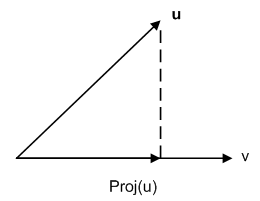
\includegraphics[bb=20 0 230 150,width=0.5\textwidth] {chap4/projection1.png}
}
\caption{Projections of u on v}
\label{figure:projection1}
\end{figure*}
Given two vectors u and v, the projection of u on v is
\[proj(u) = |u|\cos\theta \cdotp {\frac{v}{|v|}}\]
Recall that the inner product of u and v is
\[vu = v^Tu = |v||u|\cos\theta\]
by eliminating $\cos\theta$, the projection can be expressed as
\[proj(u) = |u| {\frac{v^Tu}{|v||u|}} {\frac{v} {|v|}} =
{\frac{v^Tu}{|v|}^2} v = {\frac{v^Tu}{v^Tv}} v\]
The first factor is really a scaler, so we could rewrite it
\[proj(u) = v {\frac{v^Tu}{v^Tv}} = {\frac{vv^T}{v^Tv}}u\]
So the project matrix on v is
\begin{equation}
P_v = {\frac{vv^T}{v^Tv}}
\end{equation}

where the denominator is just a scaler. Several properties of P
\begin{itemize}
\item P is symmetric, \(P^T = P\).
\item P is idempotent, \(P^2 = P\).
\end{itemize}
In numerical practice, when we deal with multiplications we don't need to store the entire P, instead we can store only the vector v. For an arbitrary vector x, 
\[Px = {{vv^T} \over {v^Tv}}x = v{{v^Tx} \over {v^Tv}} = 
{{v^Tx} \over {v^Tv}}v\]
The left factor of the above is purely a number. Similarly
\[x^TP = x^T {{vv^T} \over {v^Tv}} = {{x^Tv} \over {v^Tv}} v^T\]
Again, the left factor is a scaler. If A is a matrix, then
\[PA = {{vv^T} \over {v^Tv}}A = {{v(v^TA)} \over {v^Tv}}\]
and
\[AP = A{{vv^T} \over {v^Tv}} = {{(Av)v^T} \over {v^Tv}}\]
These formulae simplify the calculations when transforming other matrices.

Interestingly, we can extend the above result to higher dimensions. For a vector u, we want to project it to a subspace.
\begin{figure*}[htp]
\centerline{
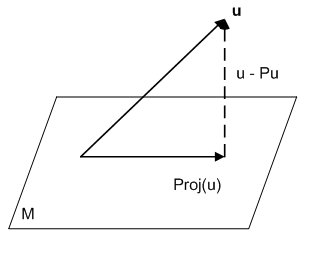
\includegraphics[bb=20 0 200 185,width=0.5\textwidth] {chap4/projection2.png}
}
\caption{Projections of u on M}
\label{figure:projection2}
\end{figure*}

\begin{lem}
Suppose \[ M = span \bigl\{v_1,\ v_2,\ \cdots,\ v_m \bigr\} \subset R^n\] where $m \leq n$ be a subspace spanned by linear independent \{$v_j$\}. The the projection matrix associated with M is
\[P = A\bigl(A^TA\bigr)^{-1}A^T\]
where $A = \bigl(v_1,\ v_2,\ \cdots,\ v_m\bigr)$, a n \texttimes m matrix, P is thus a n \texttimes n matrix. The matrix $\bigl(A^TA\bigr)^{-1}A^T$ is the pseudo inverse of A, denoted by $A^+$.
\end{lem}
\begin{proof}: For any vector u, 
\[Pu = A\bigl(A^TA\bigr)^{-1}A^Tu = A\Bigl[\bigl(A^TA\bigr)^{-1}A^Tu\Bigr] \triangleq Aw\]
So
\[Pu = (v_1,\ v_2,\ \cdots,\ v_m)
\left( \begin{array}{c} w_1\\ w_2\\ \vdots\\ w_m\\ \end{array} \right)
= \sum_{i=1}^m w_iv_i \in M \]
Next we need to prove that $u-Pu$ is perpendicular to $M$. In fact
\[A^T(u-Pu) = A^Tu - A^TPu = A^Tu - A^TA\bigl(A^TA\bigr)^{-1}A^Tu = A^Tu - A^Tu = 0\]
So $u-Pu$ is perpendicular to all ${v_j}$ and thus to $M$ too. 
It is easy to verify that $Pu$ and $u - Pu$ are perpendicular too
\[(Pu)^T(u-Pu) = u^TP^T(u-Pu) = u^TP^Tu - u^TP^TPu = 0\]
because $P^T = P$ and $P^2 = P$.
\end{proof}
Another interesting fact is the following.
\begin{figure*}[htp]
\centerline{
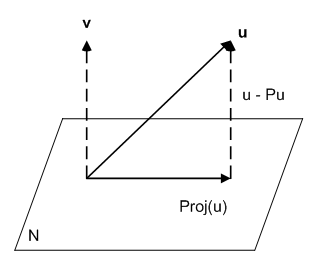
\includegraphics[bb=20 0 200 200,width=0.5\textwidth] {chap4/projection3.png}
}
\caption{Projections of u on N}
\label{figure:projection3}
\end{figure*}

\begin{lem}
Suppose $v_1,\ v_2,\ \cdots,\ v_m \in R^n$ be linear independent and $m \leq n$, let \[A = \bigl(v_1^T,\ v_2^T,\ \cdots,\ v_m^T\bigr)\] be a m \texttimes n matrix. Now consider the following subspace: \[N = \bigl\{\ x\ |\ Ax=0\ \bigr\}\] the perpendicular subspace to all $\bigl\{v_j\bigr\}$, i.e., \(N = span\bigl\{\ v_j\ |\ j=1,\ 2,\ \cdots\ m\bigr\}^\bot\). The projection matrix on N is given by
\[P = I - A^T\bigl(AA^T\bigr)^{-1}A\]
where I is the m \texttimes m identity matrix.
\end{lem}
\begin{proof}: For any vector u, 
\[A(Pu) = A\bigl(I - A^T\bigl(AA^T\bigr)^{-1}A\bigr)u = Au - AA^T\bigl(AA^T\bigr)^{-1}Au 
= Au - Au = 0\]
It implies that Pu lies in N. Furthermore, 
\[ u-Pu = A^T\left(AA^T\right)^{-1}Au \triangleq A^Tw = \bigl(v_1,\ v_2,\ \cdots\ v_m\bigr)
\left( \begin{array}{c} w_1\\ w_2\\ \vdots\\ w_m\\ \end{array} \right)
=\sum_{i=1}^m w_iv_i\]
It implies that u-Pu lies in $span\bigl\{v_i\bigr\}$ and perpendicular to N.
\end{proof}

\subsection{Reflection}
Given a vector $v$, let $M = span\bigl\{v\bigr\}^\bot$, the perpendicular space to $v$. For any vector $u$, the reflection of $u$ through M is given by
\[refl(u) = u - 2\ proj(u) = u - 2 {{vv^T} \over {v^Tv}}u =
(I - 2{{vv^T} \over {v^Tv}})u\]
\begin{figure*}[htp]
\centerline{
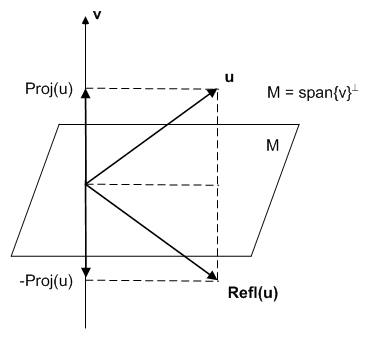
\includegraphics[bb=20 0 200 250,width=0.5\textwidth] {chap4/reflection.png}
}
\caption{Reflection of u through M}
\label{figure:reflection}
\end{figure*}
Here we use the result from last section. So the reflection matrix for M is 
\begin{equation}
Q_v = I - 2{{vv^T} \over {v^Tv}}
\end{equation}
It is easy to verify these properties:
\begin{itemize}
\item Q is symmetric, i.e., $Q^T = Q$.
\item Q is orthogonal, i.e., $Q^TQ = I$.
\item Q is involuntary, i.e., $Q^2 = I$, reflecting a vector twice should get back to the original vector.
\end{itemize}
Similar to the projection case, in numerical practice, we need to store only the vector v when applying the reflection to a vector or a matrix.

The following are several useful facts, the first one is used in the QR decomposition, the second one is used in the SVD, and the third one is used when we accumulate Householder matrices.

\begin{lem}
Given two vectors x and y with same norm, the reflection matrix that maps x to y is $Q_{x-y}$.
\end{lem}
\begin{proof}: From the above picture, if we treat u as x and refl(u) as y, it's easy to see x-y = 2proj(u) is parallel to v.
\end{proof}
If x and y don't have same norm, we could normalize both vectors first.

A typical usage of this lemma is to map a given vector to a vector of our choice, such as $e_1$, the basis in $R^n$, so that we can eliminate all components along other basis. Repeating this step we can transform a matrix to a triangular matrix.

\begin{lem}
Let x be a vector in $R^n$. For any k with $1 \leq k \leq n-2$, we can find a vector $u_k$ such that
\[Q_{u_k}x = Q_{u_k}
\left( \begin{array}{c} x_1\\ x_2\\ \vdots\\ x_k\\ \vdots\\ x_n\\ \end{array} \right) = 
\left( \begin{array}{c} x_1\\ x_2\\ \vdots\\ x_k\\ -S\\ 0\\ \vdots\\ 0\\ \end{array} \right)
\triangleq = y
\]
This means we can eliminate all components but the first two in x.
\end{lem}
\begin{proof}
If we pick 
\[S^2 = x_{k+1}^2 + x_{k+2}^2 + \cdots + x_{n}^2\]
Then x and y have the same norm. By the first lemma, 
\[u_k = x - y =
\left( \begin{array}{c} x_1\\ x_2\\ \vdots\\ x_k\\ x_{k+1}\\ x_{k+2}\\ \vdots\\ x_n\\ \end{array} \right) -
\left( \begin{array}{c} x_1\\ x_2\\ \vdots\\ x_k\\ -S\\ 0\\ \vdots\\ 0\\ \end{array} \right) =
\left( \begin{array}{c} 0\\ 0\\ \vdots\\ 0\\  x_{k+1}+S\\ x_{k+2}\\ \vdots\\ x_n\\ \end{array} \right)
\]
To avoid rounding error, the sign of S is chosen to be the same as $x_{k+1}$. Furthermore, it is easy to verify
\[ {\bigl|u_k\bigr|}_2^2 = (x_{k+1} + S)^2 + x_{k+2}^2 + \cdots + x_{n}^2
=2x_{k+1}S + 2S^2\]
\end{proof}

Lemma 3.

\subsection{Rotation}
Givens rotation matrix is defined as
\[G(i, j, c, s) = \ \ \ \bordermatrix{
    & & & & i & & & & j\cr
    & 1 \cr
    & & . \cr
    & & & 1 \cr
  i & & & & c & . & . & . & s \cr
    & & & & . & 1 \cr
    & & & & . & & . \cr
    & & & & . & & & 1 \cr
  j & & & & -s & . & . & . & c \cr
    & & & & & & & & & 1 \cr
    & & & & & & & & & & .\cr
    & & & & & & & & & & & 1\cr
}
\]
where $c^2 + s^2 = 1$. Every rotation can be decomposed into a product of a series of the above rotations.

The Householder matrix is a reflection because \(det(Q_v) = -1\). Then \(-Q_v\) is a rotation(with the angle \(\pi\)).

The Jacobi rotation is a similar transformation using G, i.e., \(G^TAG\). See the link.
\section{QR decomposition}
Let A be a n \texttimes m matrix with n > m and \(rank(A) = m\), the QR decomposition of A is \[ A = Q R \] where Q is a m \texttimes n orthogonal matrix, i.e., \(Q^TQ = I_n\), the n \texttimes n identity matrix and R is an n \texttimes n upper triangular matrix. Denote A as \[A = \bigl(\vec{a_1},\ \vec{a_2},\ \cdots,\ \vec{a_m}\bigr)\] where all \(\vec{a_j}\) are linear independent in \(R^n\) with basis $\bigl\{\vec{e_1},\ \vec{e_2},\ \cdots,\ \vec{e_n}\bigr\}$ and 
\[ \vec{a_j} = \left( \begin{array}{c} a_{1j}\\ a_{2j}\\ \vdots\\ a_{nj}\\ \end{array} \right) \] The QR algorithm, using Householder transformations, is based on the Lemma 1. After the execution, R is stored in the strictly upper triangular portion of A and R's diagonal cells are stored in a separate array. Q is stored in the lower triangular portion indirectly, actually, the vectors generating the Householder transformations are stored. In order to get Q we need to multiply these Householder transformations together. For all j, we work on the sub-matrix from j to m:
\begin{enumerate}
\item compute \(|\vec{a_j}|\), the 2-norm, square root of the sum of all components, \[\sqrt{\sum_{i=1}^{n}{a_{ij}}}\] We further select the norm to have the same sign as \(a_{jj}\) to avoid the rounding error with subtractions in the step 3.
\item overwrite \(|\vec{a_j}|\) with \(\vec{a_j} \over |\vec{a_j}|\) such that now \(\vec{a_j}\) is a unit vector. Note that we are working on the sub vector below the diagonal.
\item construct the Householder transformation for the jth sub-column so that it is mapped to \(\vec{e_j}\), the jth axis in \(R_n\). By Lemma 1, the transformation is 
\[Q_v = I - 2 {{\vec{v} \vec{v}^T} \over {\vec{v}^T \vec{v}}}\] 
where \(\vec{v} = \vec{a_j} + \vec{e_j}\). Note that \(vec{v}\) is the same as \(vec{a_j}\) except the first component is \(a_{jj} + 1\). So we just overwrite the first component of \(\vec{a_j}\) with \(a_{jj} + 1\) and thus now the jth column is \(\vec{v}\). This value will be used in the next step. As we progress j from 1 to m, the vector v has the form \(\left(0,\ 0,\ \cdots,\ v_j,\ v_{j+1},\  \cdots,\ v_n\right)\), i.e., anything above the diagonal is zero. 
\item Note that \(\vec{a_j}\) now is a unit vector, in the \(Q_v\) expression above, 
\[\vec{v}^T \vec{v} = \bigl(\vec{a_j} + \vec{e_j}\bigr)^T\bigl(\vec{a_j} + \vec{e_j}\bigr) = 
1 + a_{jj} + a_{jj} + 1 = 2\bigl(a_{jj} + 1\bigr) = 2v_j\]
So now \(Q_v\) can be expressed 
\[Q_v = I - 2 {{\vec{v} \vec{v}^T} \over {\vec{v}^T \vec{v}}} =
I - 2  {{\vec{v} \vec{v}^T} \over {2v_j}} = 
I - {{\vec{v} \vec{v}^T} \over {v_j}}\] 
where \(v_j\) is the overwritten value stored from the step 3.
\item We leave the jth column with the vector \(\vec{v}\), and apply the Householder transformation \(Q_v\) to the rest of the columns using the formula:
\[Qx = \Bigl(I - {{\vec{v} \vec{v}^T} \over v_j}\Bigr)x = 
x - {{\vec{v}^Tx} \over v_j}\vec{v}\] 
which is just a difference of two vectors x and v with a scaler.
\item store the norm from step 1 in a separate vector, this is part of the upper triangular matrix R because \(Q\vec{a_j} = |\vec{a_j}|e_j\)
\end{enumerate}
Since we store all the vectors v's in the lower portion of A, we need to multiply them to get Q.

\section{Singular Value Decomposition}
The common practice of SVD is to decompose the given matrix to a bidiagonal matrix, then compute the singular values of the reduced bidiagonal matrix.

\section{Eigen Decomposition}
scaling
\section{Reference}

For mathematical treatment, 
\begin{itemize}
\item Matrix Analysis, Horn and Johnson
\item Topics in Matrix Analysis, Horn and Johnson
\item 
\end{itemize}

For numerical algorithms
\begin{itemize}

\item Lapack documents: http://www.netlib.org/lapack/lawns/downloads/
\item Matrix Perturbation Theory, Stewart and Sun
\item Matrix Algorithms, G.W. Stewart
\item Fundamentals of Matrix Computations, D. Watkins
\end{itemize}

\begin{thebibliography}{99}

% >>>>>>>>> Book examples <<<<<<<<<
\bibitem{Demmel@1997} Demmel, J.W., {\itshape Applied Numerical Linear Algebra},
 SIAM, 1997.
\bibitem{GolubLoan} Golub, G.H., Loan, C.F., {\itshape Matrix Computations},
 3rd Edition, The Johns Hopkins University Press, 1996.
\bibitem{NumericalRecipes} Teukolsky, A., Vetterling, W.T., Flannery, B.P., {\itshape Numerical Recipes}, 3rd Edition, Cambridge University Press, 1997
\bibitem{NumericalAlgoriths} Higham, N.J., {\itshape Accuracy and Stability of Numerical Algorithms}, SIAM, 1996
\bibitem{Sparse} Sparse matrix
\bibitem{Lawn95} Lawn 95.


\end{thebibliography}


% *************** Bibliography ***************
%\bibliographystyle{plain}
%{\small\bibliography{Design_And_Implementation}}

\backmatter

\end{document}
